% !TeX spellcheck = en_EN
\documentclass[final, a4paper, 9.5pt]{article}
\usepackage[margin=2cm]{geometry}
\usepackage[english]{babel}
\usepackage[utf8]{inputenc}
\usepackage[T1]{fontenc}
\usepackage{fontspec}
\usepackage{float}
\usepackage{dirtytalk}
\usepackage{multicol}
\usepackage{sectsty}
\usepackage{hyperref}
\usepackage{graphicx}
\usepackage{caption}
\usepackage{qrcode}

\newenvironment{Figure}
  {\par\medskip\noindent\minipage{\linewidth}}
  {\endminipage\par\medskip}

\sectionfont{\fontsize{9}{12}\selectfont}

\begin{document}

% *** HEADER
\noindent
\large\textbf{Debate Project --- Final Paper} \hfill \textbf{KOCAK Mikail} \\
\normalsize Mme. Nicole Kirsch \hfill December 2018 
~\\

{\centering \Large

``\emph{Is the cloud computing a good or a bad thing?}"

}
~

% *** INTRODUCTION
This paper is the final personal response about about the above topic, after researches, and thus, fact checking. This paper is divided into multiple sections that presents a single matter, with my initial stance without any researches. And then, what I, and we, have found and discussed that have or could have changed my stance on the matter.

% *** CONTENT
\begin{multicols}{2}

% ****** SECTION
\section*{Cloud Computing Requires a Lot of Power}
This is a common thing to hear and to say. Which is true, handling a huge traffic load is not power-free, for example, each seconds, a thousands of machines are handling \cite{google_searches}:
\begin{itemize}
    \item 8,288 tweets;
    \item 71,071 Google search queries;
    \item 76,547 YouTube videos viewed;
    \item 2,751,032 Emails (67\% is spam);
    \item 65,120 GB of Internet traffic.
\end{itemize}

I, personally know, from paste researches, that cloud enterprises, independent researchers and engineers are investing a lot into R\&D to lower the power usage of the machines and the power required to manufacture them. One of the objectives being to limit waste, which requires a lot of energy. A good example, are the ARM processors that are more and more commonly used for servers and mobiles, that keep on getting more powerful while using way less power.

When doing our researches, we found that the internet and intranet traffic keep on growing, but the power usage is almost remaining still as results of numerous R\&D \cite{traffic_growth}. Below, we made a graphic summarizing this fact.
\begin{Figure}
    \centering
    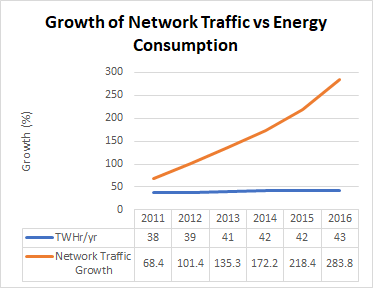
\includegraphics[width=\linewidth]{figures/cloudgrowth.png}
    \captionof{figure}{
        \scriptsize Electricity Consumption of the data-centers, including the power usage of manufacturing the hardware (TWh/yr) vs Growth in Core Network Traffic (including traffic within data centers), where \char`\~70\% of total traffic is between data centers.}
\end{Figure}

So, we have been proven that it doesn't cost that much, and hopefully, the power usage trend could even start lowering despite the user count going up.

% ****** SECTION
\section*{Users Have No Control}
A huge concern in cloud computing, is the fact the users have no control. I personally thought, and still think, that it's a huge security concerns, but after researches, it seems to be a great solution for non-enterprise users, especially 'lambda' users. We raised the following positive points \cite{good_bad_ugly}:

\begin{enumerate}
    \item \emph{Lambda users} don't have to worry about their privacy, they assume their data is safe and monitored against intrusions;
    \item Users don't have to upgrade and invest into hardware. Thus, it's cheap, and protect the Earth against waste; especially as most of the hardware parts can last for at least 10 to 20 years without any issues, but most users change and trash them very often;
    \item \emph{Lambda users} don't know how to protect their data, the cloud does it for them.
\end{enumerate}

But we also found that it's still true that users should be scared, especially enterprise users. As I was thinking before doing the researches: the cloud is, and should be treated as a trust based solution; where have a service that works, that we are happy with... but, that can, any day go south if the service wasn't properly maintained and monitored, which happens often. Enterprises cannot assume that a service is reliable, they need to be certain. Our researches have confirmed those facts \cite{the_ugly}. Often, enterprises are willing to pay good money to have the cloud service engaging itself to give a maximal security, availability and support. Which, gives a low-cost maximal productivity for the enterprise.

\end{multicols}

\newpage

% *** BIBLIOGRAPHY
\begin{thebibliography}{9}
\bibitem{google_searches}
    \emph{Google Search Statistics}  (\href{http://www.internetlivestats.com/google-search-statistics/}{internetlivestats.com}) [last acceded: the 2th Nov., 2018];
    
\bibitem{traffic_growth}
    \emph{Emerging trends in electricity consumption for consumer ICT} --
    Andrae, Anders; Corcoran, Peter M., published in 2013,
    (\href{https://aran.library.nuigalway.ie/bitstream/handle/10379/3563/CA_MainArticle14_all-v02.pdf?sequence=4&isAllowed=y}{aran.library.nuigalway.ie}) [last acceded: the 2th Nov., 2018];
    
\bibitem{good_bad_ugly}
    \emph{Cloud Computing: The Good, The Bad, \& The Ugly} --
    James Wilkinson, published the 13th Sept., 2016,
    (\href{https://strategiccfo.com/cloud-computing-good-bad-ugly/}{strategiccfo.com}) [last acceded: the 2th Nov., 2018];
    
\bibitem{the_ugly}
    \emph{8 Reasons to Fear Cloud Computing} --
    Sara Angeles, Business News Daily Staff Writer, published the 1st Oct., 2013,
    (\href{https://www.businessnewsdaily.com/5215-dangers-cloud-computing.html}{businessnewsdaily.com}) [last acceded: the 2th Nov., 2018];

\end{thebibliography}

\end{document}
